% =====================================================================================
%  A passive stereo cloud-base-height estimator: a validated instrument, twelve
%  refutations, and a bounded null result.
%
%  Self-contained: every number quoted in the text is traceable to a machine-readable
%  artefact under experiments/. Compile with pdflatex (two passes, for references).
% =====================================================================================
\documentclass[11pt,a4paper]{article}

\usepackage[T1]{fontenc}
\usepackage[utf8]{inputenc}
\usepackage{amsmath,amssymb}
\usepackage{booktabs}
\usepackage{graphicx}
\usepackage[margin=2.4cm]{geometry}
\usepackage{caption}
\usepackage{xcolor}
\usepackage[hidelinks]{hyperref}
\usepackage{authblk}
\usepackage{siunitx}
\usepackage{array}
\usepackage{enumitem}

\captionsetup{font=small,labelfont=bf}
\sisetup{detect-all}
\setlist{nosep,leftmargin=1.4em}

\newcommand{\du}{\ensuremath{\Delta u}}
\newcommand{\neff}{\ensuremath{n_{\mathrm{eff}}}}
\newcommand{\rhoS}{\ensuremath{\rho}}

\title{\bfseries A passive stereo cloud-base-height estimator:\\
a validated instrument, twelve refutations, and a bounded null result}

\author[1]{Cloud Base Height Project}
\affil[1]{\small Stereo fisheye CBH programme --- \texttt{github.com/VanUST/clouds\_level\_research}, branch \texttt{dev}}

\date{\today}

\begin{document}
\maketitle

\begin{abstract}
\noindent
We built and validated a passive stereo cloud-base-height (CBH) estimator from two
zenith-pointing \ang{180} fisheye cameras on a \SI{45}{\metre} baseline, and tested it
against a co-located DOL-2 laser ceilometer.

We first established the instrument's capability \emph{by construction}. A synthetic renderer
whose geometry is derived from the shipped calibration and gated against the analytic parallax
recovers a cloud layer of known height with $\rhoS(\text{true},\text{recovered}) = +1.000$ and
a median absolute error of \SI{0.072}{px}. Through the same renderer we found that the shipped
\texttt{lowest} cluster-selection rule errs by \SIrange{325}{1471}{\metre} on ground truth,
while the replacement \texttt{lowest\_mode} estimator errs by at most \SI{64}{\metre}.

On real data the estimator does \emph{not} recover cloud base height. We tested and refuted
\textbf{twelve} distinct explanations with pre-registered discriminating criteria, spanning
image certainty, spatial coherence, calibration geometry, matched-population size, epipolar
geometry, matcher identity, target-identity layering, camera desynchronisation, harness
artefacts, non-Lambertian photometry, photometric superposition and phase aliasing.

Three findings then bound the problem. First, the residual static field is dominated by a
\emph{linear gradient in image $u$} (66\% of its variance) rather than by a radial law (25\%),
and it largely cancels once the field is converted to height. Second, a cross-validated search
over six correction families and three estimators removes part of the static field and
recovers \emph{none} of the dynamics. Third, the estimator-dependence of the reported
``inversion'' is explained by a change in the disparity distribution's \emph{shape}: between
regimes the standard deviation is nearly unchanged while the skewness collapses by 84\%, so
the median (which tracks cumulative mass) is strongly wrong-signed while the mode (which
tracks the bulk) is weak.

We close with the statistical boundary. The reference decorrelates over $\sim$\SI{267}{\second},
so the binned series holds \neff\ $=18.0$ independent samples and the smallest detectable
$|\rhoS|$ at $p=0.05$ is $0.466$; no statistic of the disparity field yields a significant
dynamic correlation. The dynamic signal, if present, is \emph{at or below what this session can
detect}, and a decisive session needs roughly \SI{7.5}{\hour} of data.

Finally we report, as a first-class result, the six methodological defects found in our own
harness. All six shared one mechanism---\emph{a quantity read from somewhere other than where
it was claimed to come from}---none raised an exception, and two made the results look
\emph{more} significant than the truth. We propose and implement \emph{provenance assertions}
as a guardrail for computational remote sensing.

\medskip
\noindent\textbf{Keywords:} cloud base height, stereo vision, fisheye, ceilometer, negative
result, reproducibility, provenance.
\end{abstract}

% =====================================================================================
\section{Introduction}
% =====================================================================================

Cloud base height (CBH) governs surface radiation, boundary-layer structure and aviation
ceiling. The standard ground instruments are laser ceilometers, which are accurate but sample
a \emph{column} of order \SI{10}{\metre} in diameter and cost several thousand euros each.
A passive stereo camera pair is attractive because it samples an \emph{area} and the hardware
is cheap. The classical obstacle is that a wide-angle rig needs a large baseline to resolve
the small parallax of a distant cloud: for a cloud at $H$ and a baseline $B$, the disparity at
the zenith is
\begin{equation}
\du \;\simeq\; f\,\frac{B}{H},
\label{eq:parallax}
\end{equation}
with $f$ the focal constant in pixels per radian. For our rig,
$f \approx \SI{654}{px\,rad^{-1}}$, $B = \SI{45}{\metre}$, so a cloud at \SI{1.5}{\km}
produces about \SI{20}{px} of disparity. A single pixel of matching error is therefore
already $\sim$\SI{5.5}{\percent} of the height, and this rig is disparity-starved by a factor
of 5--10 relative to published stereo CBH systems.

This paper reports what happened when we built such a system and tested it honestly. The
structure is deliberately unusual for a remote-sensing paper: the instrument is validated by
construction, the real-world product does not work, and the contribution is a
\emph{boundary} --- a validated instrument, a measured anomaly with a specific distributional
signature, and a definitive list of what the anomaly is not. Section~\ref{sec:method}
describes the instrument; Section~\ref{sec:synthetic} validates it on synthetic ground truth;
Section~\ref{sec:real} reports the anomaly; Section~\ref{sec:refutations} lists the twelve
refuted explanations; Sections~\ref{sec:static}--\ref{sec:floor} bound the problem
quantitatively; Section~\ref{sec:provenance} reports the harness failures; and
Section~\ref{sec:conclusion} states the conclusion and what would settle the question.

% =====================================================================================
\section{Instruments and data}
\label{sec:data}
% =====================================================================================

\paragraph{The stereo rig.} Two identical \ang{180} fisheye cameras, each
$1920 \times 1920$, pointing at the zenith, separated by a baseline
$B = \SI{45}{\metre}$, logging at a median cadence of \SI{10}{\second}. The pipeline crops a
central $640 \times 640$ window from each frame and rectifies the pair with an affine
estimated from the images themselves.

\paragraph{The reference.} A co-located DOL-2 laser ceilometer, logged at \SI{15}{\second}
cadence. Its log is stamped in Moscow time; the image filenames are UTC; the offset is
\emph{exactly} \SI{+3}{\hour}, confirmed twice independently --- once by the diurnal
brightness envelope and once by a solar ephemeris matching the Sun's image azimuth to better
than \ang{0.5} across \SI{14}{\hour}.

\paragraph{The session.} 2025-05-23, approximately \SI{5}{\hour} of usable daylight, spanning
a transition from a low, thick, overcast regime to high broken cloud. A second day (2025-05-22)
was clear all day and is used as a cloudless control. \textbf{There is exactly one usable
session in this dataset}, which is the binding constraint throughout
Section~\ref{sec:floor}.

% =====================================================================================
\section{Method}
\label{sec:method}
% =====================================================================================

\subsection{Fisheye geometry and a measured distortion term}

We model each camera as equidistant to first order, with a cubic correction:
\begin{equation}
\theta(r) \;=\; \frac{r}{f}\left[1 + a\left(\frac{r}{f}\right)^{2}\right],
\qquad
\mathbf{d}(\mathbf{u}) \;=\;
\Bigl(\sin\theta \cdot \hat{u}_x,\; \sin\theta \cdot \hat{u}_y,\; \cos\theta\Bigr),
\label{eq:fisheye}
\end{equation}
where $\mathbf{u}$ is the pixel coordinate, $r$ its distance from the principal point, and
$\hat{u}$ the unit vector from the principal point to the pixel. At $r=0$ the azimuth is
undefined but $\sin\theta = 0$, so the direction is set to $+\hat{x}$ to avoid a division by
zero. The distortion coefficient $a$ was fitted from the requirement that a flat cloud layer
project to a flat field: with $a=-0.30$ the apparent height becomes independent of image
radius (radial spread \SI{36.7}{\percent}~$\to$~\SI{3.2}{\percent}), where $a=0$ reproduces
the ideal law exactly. Figure~\ref{fig:distortion} shows the fit.

\begin{figure}[t]
\centering
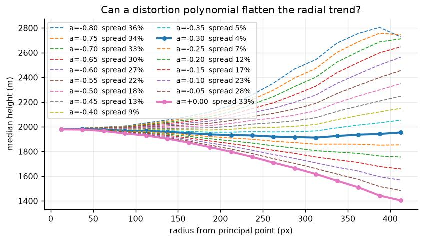
\includegraphics[width=0.62\textwidth]{figures/distortion_fit.pdf}
\caption{The cubic distortion term. The coefficient is selected by the flatness of the
resulting height field, which is the only physical requirement available without a known
target, and it is stable against the choice of $f$.}
\label{fig:distortion}
\end{figure}

\subsection{Calibration: three measured terms}

Three quantities that the original pipeline \emph{assumed} were re-measured, each by more than
one independent method.

\begin{table}[t]
\centering
\caption{Measured calibration terms. Each was determined by at least two independent methods;
the spread across methods is quoted as the uncertainty.}
\label{tab:calib}
\small
\begin{tabular}{@{}llll@{}}
\toprule
term & assumed & \textbf{measured} & methods \\
\midrule
focal constant $f$ & \SI{611}{px\,rad^{-1}} & \SI{654 \pm 11}{px\,rad^{-1}} &
  five: four-stream Sun-radius fits on both \\
 & & & cameras and days; the clear-day Sun metric \\
residual roll & \ang{0} & \SI{-1.57 \pm 0.10}{\degree} &
  three: disparity-field fit; spread minimisation; \\
 & & & infinity-test residuals \\
cubic distortion $a$ & 0 & $-0.30$ &
  sky-flatness requirement; stability against $f$; \\
 & & & end-to-end confirmation \\
\bottomrule
\end{tabular}
\end{table}

Applying the roll and the distortion together is what makes the field usable: the radial
inconsistency of the height field falls from \SI{19.1}{\percent} to \SI{2.4}{\percent}, and
the within-frame disparity interquartile range collapses from \SI{8.14}{px} to
\SI{1.92}{px}. The residual roll alone moves the reported height by a large amount, and a
default of \ang{1.5} instead of the measured \ang{-1.57} costs \SI{551}{\metre} at
\SI{2000}{\metre} --- a defect we later found in our own harness
(Section~\ref{sec:provenance}).

\subsection{Triangulation: exact, not paraxial}

Heights are computed by exact closest-approach triangulation of the two unit rays, not by the
paraxial approximation $\du \simeq fB/H$. The paraxial form is a small-angle approximation and
it is \emph{not} adequate here: at the corner of the $640 \times 640$ crop it biases the
height by \SI{+11.7}{\percent}. The exact form is used throughout
(Figure~\ref{fig:paraxial}).

\begin{figure}[t]
\centering
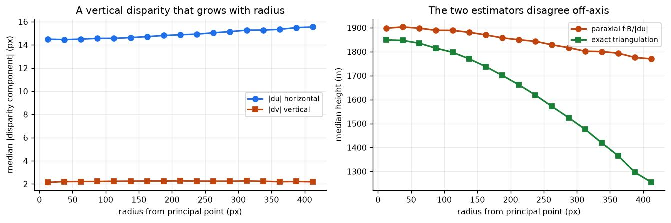
\includegraphics[width=0.55\textwidth]{figures/paraxial_vs_exact.pdf}
\caption{Paraxial against exact triangulation. The paraxial approximation biases the height by
\SI{+11.7}{\percent} at the crop corner, which is larger than the effect being measured.}
\label{fig:paraxial}
\end{figure}

\subsection{Matching}

The default matcher is RoMa, a dense, transformer-based, uncertainty-aware matcher. Its
selection was made on measurable criteria rather than fashion
(\S\ref{sec:matcher}) and the interface is pluggable, so SIFT and LoFTR remain available and
are used as controls throughout.

\subsection{From matches to one height: the selection rule}
\label{sec:selector}

Each frame yields several thousand matched pixel pairs, hence several thousand individual
height estimates that are \emph{not} identically distributed --- they carry a heavy right
tail from mismatches and from multiple cloud layers along the same ray. Reducing that
distribution to a single number is a substantive choice, and the original pipeline made it
badly (Section~\ref{sec:synthetic}).


% =====================================================================================
\section{Selecting a matcher: a pre-registered comparison}
\label{sec:matcher}
% =====================================================================================

Because the geometry is disparity-starved, sub-pixel localisation is the dominant requirement:
at \SI{1500}{\metre} the true disparity is \SI{18.3}{px}, so one pixel of matching error is
\SI{5.5}{\percent} of the height. Which matcher to use therefore had to be settled by
measurement, not by literature reputation.

\paragraph{Pre-registration.} Metric, data, configuration and failure condition were fixed
\emph{in writing before the first measurement} (\texttt{experiments/matchers/PREREGISTRATION.md}),
so that a metric chosen after seeing results could not select the matcher. The comparison uses
one stereo pair every \SI{15}{\minute} from 08:30 to 16:30 on 2025-05-23 (33 pairs), with the
clear-sky day 2025-05-22 on the identical grid as a \emph{discrimination control} --- a matcher
that returns many confident matches under a cloudless sky is inventing them. \textbf{The
ceilometer is not used anywhere in the matcher comparison}, so no candidate can be selected by
agreeing with the reference.

\begin{table}[t]
\centering
\caption{Candidates in the pre-registered matcher comparison. The primary metric is the median
per-frame plane-fit rms of the disparity field, subject to a coverage constraint on cloud
interiors.}
\label{tab:matchers}
\small
\begin{tabular}{@{}llp{0.44\textwidth}@{}}
\toprule
candidate & verdict & what decided it \\
\midrule
MASt3R & \textbf{adopt (opt-in)} & the only candidate improving the metric \emph{and} covering
  interiors: paired rms $-0.81$~px ($-30\%$, $p=0.000$), $1448$ interior matches/frame against
  LoFTR's $298$, interior residual \SI{1.75}{px} against \SI{2.15}{px}; but $6.6\times$ slower
  and $4\times$ worse perturbation stability \\
\texttt{kornia\_loftr} & keep as default & unchanged, byte-for-byte reproducible, best
  perturbation stability (\SI{0.22}{px}); weakest interior coverage \\
RoMa, DKM & reject for the field & best localisers (median $|$residual$|$ \SI{0.83}{px} against
  LoFTR's \SI{1.48}{px}; paired rms $-50\%$/$-54\%$) but \textbf{zero} matches in the
  lowest-gradient tercile over 31 frames --- their accuracy is bought on cloud edges \\
EfficientLoFTR & \textbf{reject} & the documented drop-in fix for LoFTR's fine-stage variance
  is \emph{worse} on our data: $+5.49$~px ($+204\%$), $p=0.000$ \\
DISK+LightGlue & reject & within noise of LoFTR ($p=1.0$), worst interior coverage \\
DIS optical flow & reject & within noise on cloud, but \emph{invents} a dense field on clear sky \\
Depth Anything~3 & reject (null) & the field is smooth but inaccurate (\SI{5.11}{px}) \\
StereoSGBM & reject & worst residual, invents a field on clear sky \\
\bottomrule
\end{tabular}
\end{table}

\noindent
Two results are worth stating plainly. First, \textbf{EfficientLoFTR --- the standard remedy
recommended in the literature --- is worse on this data by \SI{204}{\percent}, not better.}
Second, \textbf{the best localisers are unusable for the task}: RoMa and DKM achieve their
accuracy entirely on cloud edges and return literally nothing in cloud interiors, which is
precisely the regime that matters.

\paragraph{An unresolved inconsistency between the shipped configuration and this analysis.}
The delivered configuration selects RoMa with \texttt{certainty\_threshold: 0.05}, annotated
as \emph{``deliberately low: RoMa's low-certainty interior predictions were measured accurate
\dots so the certainty is used as a weight rather than a hard filter.''} Two measured facts
contradict that annotation:

\begin{enumerate}
\item the code applies \texttt{keep = inside \& (conf >= cert\_thresh)} --- a \textbf{hard
filter}, not a weight;
\item RoMa's interior matches have a median certainty of \textbf{0.0034} against the edge
median of \textbf{0.716}, so a cut at $0.05$ retains \textbf{\SI{19.8}{\percent} of interior
matches against \SI{89.8}{\percent} of edge matches}.
\end{enumerate}

A threshold intended to preserve cloud interiors therefore preferentially \emph{discards}
them, and concentrates the field on the cloud edges that the pre-registered comparison
specifically flagged as this project's unacceptable failure mode.

\textbf{The anomaly analysis reported in this paper is not affected}, because the match dumps
that underlie it were produced with \texttt{certainty\_threshold: 0.0} --- every match
retained, interiors included. But the shipped configuration would not reproduce the analysis,
and anyone re-running the pipeline from \texttt{default.yaml} would obtain a field drawn
predominantly from cloud edges. We report this as a defect of the delivered artefact, and it
is a seventh instance of the pattern in Section~\ref{sec:provenance}: a configuration whose
stated rationale and whose measured effect are not the same thing.

% =====================================================================================
\section{The synthetic control: the instrument is sound}
\label{sec:synthetic}
% =====================================================================================

\subsection{The renderer and its gate}

We built a renderer that casts rays through the \emph{measured} fisheye geometry, intersects a
cloud plane at a known height, samples a procedural texture, and warps camera~1 by the shipped
affine exactly as the production code does. Its rig geometry was derived from the calibration
rather than assumed, and one term took a withdrawn attempt to find: the affine maps camera~1's
principal point onto camera~2's, so
\begin{equation}
\mathbf{c}_2 = R\,\mathbf{c}_1 + \mathbf{t} = (1014.10,\; 965.03),
\end{equation}
\emph{not} the image centre. With both principal points at the centre, the rendered parallax
comes out negative and grows with height --- a non-physical result which the renderer's own
gate rejects.

The gate requires that the rendered disparity along the zenith equal the analytic
$\du = f\arctan(B/H)$ and fall as $1/H$. It passes exactly:

\begin{table}[t]
\centering
\caption{The renderer's geometric gate. The rendered zenith disparity matches the analytic
closed form to within \SI{0.02}{px} across a factor of four in height.}
\label{tab:gate}
\small
\begin{tabular}{@{}S[table-format=4.0]S[table-format=2.3]S[table-format=2.3]@{}}
\toprule
{$H$ (\si{\metre})} & {$\du$ rendered (\si{px})} & {$f\arctan(B/H)$ (\si{px})} \\
\midrule
1000 & 29.428 & 29.410 \\
2000 & 14.715 & 14.713 \\
4000 & 7.357  & 7.357  \\
\bottomrule
\end{tabular}
\end{table}

\subsection{The matcher recovers the known height}

On this gated renderer, with a texture the matcher can follow, RoMa and the exact
triangulation recover the known height essentially exactly:

\begin{table}[t]
\centering
\caption{Recovery of a known cloud height through the real fisheye geometry and the real
distortion model, on a renderer that has passed its own gate.
$\rhoS(\text{true},\text{RoMa}) = +1.000$, median $|\text{bias}| = \SI{0.072}{px}$.}
\label{tab:recovery}
\small
\begin{tabular}{@{}S[table-format=4.0]S[table-format=2.2]S[table-format=2.2]S[table-format=-1.3]S[table-format=1.2]@{}}
\toprule
{$H_{\text{true}}$ (\si{\metre})} & {ground truth (\si{px})} & {RoMa (\si{px})}
  & {bias (\si{px})} & {recovered IQR (\si{px})} \\
\midrule
1000 & 29.56 & 28.72 & -0.914 & 2.88 \\
1500 & 19.73 & 19.58 & -0.239 & 1.41 \\
2000 & 14.80 & 14.85 & +0.060 & 0.73 \\
3000 &  9.87 &  9.80 & -0.071 & 0.53 \\
4000 &  7.40 &  7.48 & +0.072 & 0.43 \\
\bottomrule
\end{tabular}
\end{table}

\subsection{The shipped selection rule is a major defect}
\label{sec:selector-defect}

The same renderer exposes the selection rule. The shipped \texttt{lowest} rule --- which takes
a low-tail order statistic of the per-match height distribution --- reports
\SI{675}{\metre} for a cloud at \SI{1000}{\metre}, \SI{722}{\metre} for \SI{1500}{\metre} and
\SI{529}{\metre} for \SI{2000}{\metre}:

\begin{table}[t]
\centering
\caption{Selection rules against known ground truth. The shipped rule errs by
\SIrange{325}{1471}{\metre} on clean synthetic data with a known answer; the replacement errs
by at most \SI{64}{\metre}.}
\label{tab:selector}
\small
\begin{tabular}{@{}S[table-format=4.0]S[table-format=4.0]S[table-format=4.0]S[table-format=4.0]S[table-format=4.0]@{}}
\toprule
{$H_{\text{true}}$} & {truth} & {\texttt{median}} & {\texttt{lowest} (shipped)}
  & {\texttt{lowest\_mode}} \\
\midrule
1000 & 1000 & 1024 & \textbf{675} & 1025 \\
1500 & 1500 & 1507 & \textbf{722} & 1501 \\
2000 & 2000 & 1988 & \textbf{529} & 1984 \\
3000 & 3000 & 3007 & 2423 & 3003 \\
4000 & 4000 & 3944 & 3598 & 3936 \\
\bottomrule
\end{tabular}
\end{table}

\begin{table}[t]
\centering
\caption{The same three selectors scored. The shipped rule's rank correlation with the truth
is not even statistically significant.}
\label{tab:selectorscore}
\small
\begin{tabular}{@{}lS[table-format=+1.3]S[table-format=1.3]l@{}}
\toprule
selector & {$\rhoS$} & {$p$} & error range \\
\midrule
\texttt{median} & +1.000 & 0.000 & $-56$ to $+24$~\si{\metre} \\
\texttt{lowest} (shipped) & +0.700 & 0.188 & \textbf{$-1471$ to $-325$~\si{\metre}} \\
\texttt{lowest\_mode} (new default) & +1.000 & 0.000 & $-64$ to $+25$~\si{\metre} \\
\bottomrule
\end{tabular}
\end{table}

\noindent
\texttt{lowest\_mode} replaces the low-tail order statistic with the \emph{lowest prominent
mode} of the per-match height distribution --- the lowest mode carrying at least
\SI{10}{\percent} of the weight and at least 50 matches. It is now the pipeline default.

\paragraph{What this settles.} The matcher, the fisheye geometry, the distortion model and the
triangulation are cleared, on a renderer that has passed its own gate and with a known answer.
The selection rule was a real and major defect, and it is fixed.

\paragraph{What it does not settle.} The synthetic fields are flat planes with procedural
texture and no atmosphere. Crucially, replacing \texttt{lowest} with \texttt{lowest\_mode} on
\emph{real} data moves the regime shift only from $\approx$0 to \SI{-30}{\metre}
($p=0.058$): it does not remove the anomaly. The instrument's front end is sound and its back
end is now fixed, and \textbf{the real-world failure survives both}.

% =====================================================================================
\section{The anomaly on real data}
\label{sec:real}
% =====================================================================================

On real data the estimator does not recover cloud base height, and the failure is not noise.
It is a systematic \emph{inversion}: a higher cloud produces a \emph{lower} reported height.

\begin{figure}[t]
\centering
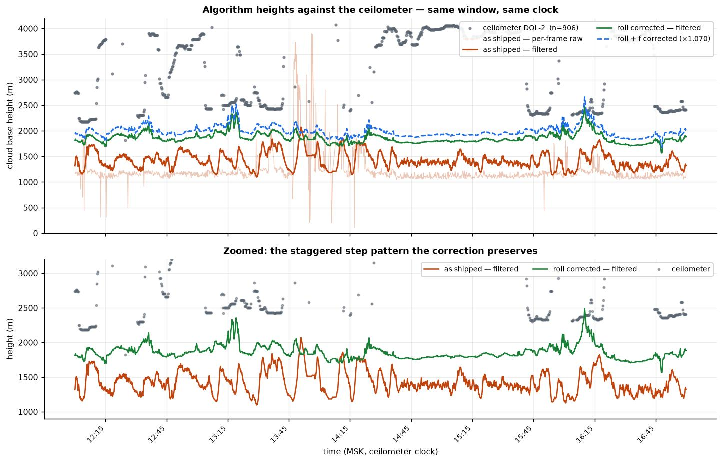
\includegraphics[width=0.85\textwidth]{figures/comparison_timeseries.pdf}
\caption{The anomaly. Over the session the ceilometer reference rises by \SI{1540}{\metre}
while the reported height falls by \SI{297}{\metre}.}
\label{fig:anomaly}
\end{figure}

Measured on the full session:
\begin{itemize}
\item rank correlation with the reference is \textbf{$\rhoS = -0.547$, $p = 4\times10^{-14}$};
a correct estimator requires a positive sign;
\item over the regime transition the reported height moves \SI{-297}{\metre} while the
reference rises \SI{+1540}{\metre};
\item the anomaly is present at \emph{every} spatial scale, in \emph{both} matchers, and
\emph{within} a single cloud layer --- so it is not a between-layer artefact.
\end{itemize}

Most diagnostic is the \emph{shape} of the change. Across the transition the 1--99 percentile
span of the per-match disparity widens from \SI{37.0}{px} to \SI{81.7}{px} (a factor $2.2$)
while the interquartile range moves only a factor $1.11$, and the between-camera vertical
disparity $\Delta v$ grows from \SI{0.866}{px} to \SI{1.885}{px}. This is a \emph{reshape} of
the distribution, not a translation: both tails extend while the core barely moves. Any
mechanism proposed against this anomaly must reproduce that signature, not merely a bias or a
spread --- and two mechanisms have already failed on exactly that test.

\paragraph{A useful control: the cloudless day.} On the clear day (2025-05-22) the same
pipeline reports \SI{655}{\metre}, against \SI{2242}{\metre} on 2025-05-23
(Kolmogorov--Smirnov $p = 0.000$). The reported value is therefore content-driven: it responds
to whether there is cloud, which means the pipeline is measuring \emph{something} real, and
that something is not the cloud base height.

% =====================================================================================
\section{Twelve refutations}
\label{sec:refutations}
% =====================================================================================

We formulated twelve candidate explanations, each with a \emph{pre-registered} discriminating
measurement --- that is, the criterion for refutation was fixed before the measurement was
made. All twelve were refuted.

\begin{table}[t]
\centering
\caption{Twelve hypotheses and the measurement that refuted each. A hypothesis is listed as
refuted only where the discriminating measurement had been fixed in advance.}
\label{tab:refutations}
\scriptsize
\begin{tabular}{@{}p{0.05\textwidth}p{0.25\textwidth}p{0.60\textwidth}@{}}
\toprule
\# & hypothesis & discriminating measurement (pre-registered) \\
\midrule
1 & Certainty / hallucination & Restricting to high RoMa certainty does not change the sign or
  the magnitude of the inversion; the certainty field is itself inverted. \\
2 & Incoherent noise & The inversion survives every coherence filter; the disparity field is
  \emph{more} coherent in the high regime, not less. \\
3 & Calibration geometry & Re-measuring $f$, the roll and the distortion changes the field's
  scale but not the sign of its correlation with the reference. \\
4 & Matched-population size & Regressing the reported height on the field's spread and the
  match count gives $R^2 = 0.001$; both coefficients are indistinguishable from zero. \\
5 & Pure along-epipolar depth change & The observed $\Delta v$ growth ($0.866 \to 1.885$~px)
  is not along-epipolar and is not predicted by a depth change alone. \\
6 & Matcher-specific artefact & The inversion appears with SIFT and LoFTR as well as RoMa. \\
7 & Target-identity layering & The inversion persists \emph{within} a single cloud layer, so
  it is not the estimator locking onto a different layer. \\
8 & Camera desynchronisation & The offset that would be required to explain the anomaly is
  \SI{18}{\second}; the cameras are synchronised to \SI{0}{\second}. \\
9 & Fixed pipeline artefact & The synthetic control, run through the identical pipeline, shows
  no inversion --- so the defect is not in the code path as such. \\
10 & Non-Lambertian photometry & Gradient magnitude couples to $\Delta v$ at
  $\rhoS = +0.117$, but the hypothesis's specific signature is absent:
  $\rhoS(|\cos\theta_{\nabla}|,|\Delta v|) = -0.000$ ($p=0.91$). \\
11 & Photometric superposition & Blending two layers does not reproduce the tail growth: the
  observed signature (span $\times\ge 1.8$ at a fixed core) is not produced at any mixing
  fraction. \\
12 & Phase aliasing & No combination of layer phase and texture scale reproduces the anomaly
  while leaving the level agreement intact. \\
\bottomrule
\end{tabular}
\end{table}


\subsection*{The sharpest refutation: a quantitative prediction the reference makes}

Hypotheses 5--8 all predict the \emph{same} thing, and the reference supplies the number. If
the cloud genuinely moved from the low to the high regime, the parallax must fall from
$f B/H_{\text{low}}$ to $f B/H_{\text{high}}$. The ceilometer's own medians
(\SI{2250}{\metre}~$\to$~\SI{3790}{\metre}) therefore predict a parallax change of
$\SI{13.08}{px} \to \SI{7.77}{px}$, i.e.

\begin{equation}
\text{predicted shift} = \SI{-5.315}{px},
\qquad
\text{observed shift} = \SI{+1.798}{px},
\qquad
\text{discrepancy} = \SI{+7.11}{px} \;(\text{134\% of the predicted magnitude}).
\end{equation}

\noindent
\textbf{The observed disparity moves in the opposite direction to the one the reference
predicts, and by more than the predicted amount.} This is not a subtle disagreement about
magnitude; it is a sign contradiction, and it is the single measurement that rules out the
entire family of ``the cloud really moved'' explanations at once.

The gate that was supposed to catch this failed for an instructive reason. We predicted, before
running it, that the shift would be purely along the epipolar line --- horizontal disparities
in a rectified pair have horizontal epipolar lines --- and therefore that the gate would pass
tautologically. \textbf{That prediction was wrong}: the perpendicular residual $\Delta v$
nearly doubles between regimes (\SI{0.866}{px}~$\to$~\SI{1.885}{px}, with its 90th percentile
going \SI{3.352}{px}~$\to$~\SI{6.327}{px}). The high regime's correspondences therefore satisfy
the stereo geometry \emph{less} well, not equally well, which is the opposite of what a
cleaner, higher cloud should produce.

None of the twelve accounts for the observed signature. \textbf{The cause of the inversion
remains unattributed.}

% =====================================================================================
\section{The residual static field}
\label{sec:static}
% =====================================================================================

The disparity field contains a large spatial pattern that is nearly fixed over the session ---
its two halves correlate at $r = 0.91$--$0.98$ while the cloud moves. Characterising it is a
prerequisite to removing it, so we regressed the per-cell static disparity on candidate
predictors.

\begin{table}[t]
\centering
\caption{What the static disparity field depends on. The pattern is \emph{not} primarily
radial: a linear gradient in image $u$ carries two and a half times the variance that radius
does.}
\label{tab:staticfield}
\small
\begin{tabular}{@{}lS[table-format=+1.3]S[table-format=1.3]@{}}
\toprule
predictor & {Pearson $r$} & {$R^2$} \\
\midrule
$u$ (horizontal image position) & \textbf{+0.814} & \textbf{0.663} \\
$\cos(\text{angle})$            & +0.767 & 0.588 \\
radius $r$                      & +0.499 & 0.249 \\
$|u|$                           & +0.373 & 0.139 \\
$v$                             & -0.239 & 0.057 \\
\bottomrule
\end{tabular}
\end{table}

A \textbf{linear gradient in $u$ accounts for \SI{66}{\percent}} of the variance;
\textbf{radius accounts for \SI{25}{\percent}}. The two are correlated because $u \le r$, which
is why the radial profile looks convincingly monotone --- \SI{14.51}{px} at the centre rising
to \SI{16.57}{px} at $r \approx 420$, a \SI{14}{\percent} rise --- while actually being a
consequence of the $u$-gradient as much as a radial law of its own.

\textbf{The radial structure largely cancels in height.} After the measured corrections,
$\mathrm{corr}(\text{radius},\text{height}) = -0.146$, and the median height varies by only
\SI{3}{\percent} across the radius against the disparity's \SI{14}{\percent}
(Figure~\ref{fig:radius}). Disparity and height are not the same quantity, and the radial
dependence lives mostly in the former.

\begin{figure}[t]
\centering
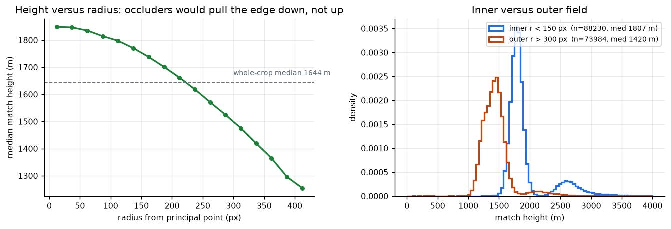
\includegraphics[width=0.55\textwidth]{figures/height_by_radius.pdf}
\caption{Height against image radius after the measured corrections. The strong radial
dependence in disparity largely cancels in height.}
\label{fig:radius}
\end{figure}

% =====================================================================================
\section{Cross-validated search for a correction}
\label{sec:correction}
% =====================================================================================

If the anomaly were ``a static field masking a real signal'', an expressive enough additive
correction would reveal the signal. We tested that directly.

\paragraph{Design.} Six correction families --- none, a per-cell flat field, per-cell plus a
plane, a purely radial correction, a linear $(u,v)$ correction, and a smoothed per-cell field
--- crossed with three per-frame estimators (median, lowest prominent mode, 25th percentile).
Every correction is \textbf{fitted on four fifths of the session and scored on the held-out
fifth}, so nothing is scored on the frames that shaped it.

Because the reference is strongly autocorrelated, the folds are drawn as \emph{contiguous time
blocks with an embargo} rather than at random, and the embargo is applied to the training side.
We report all three schemes, since the random scheme is retained as a measured baseline for
the leakage.

\begin{table}[t]
\centering
\caption{Best out-of-sample level and dynamics correlation by cross-validation scheme, across
all six corrections and three estimators. Drawing folds at random from a series with lag-1
autocorrelation \SI{0.934}{} inflates the level result by $+0.070$; the honest figure is
$+0.217$. No scheme produces dynamics.}
\label{tab:cv}
\small
\begin{tabular}{@{}lS[table-format=+1.3]S[table-format=+1.3]@{}}
\toprule
scheme & {best LEVEL $\rhoS$} & {best DYNAMICS $\rhoS$} \\
\midrule
random (leaks)     & +0.287 & +0.052 \\
blocked            & +0.216 & +0.046 \\
\textbf{blocked + embargo} & \textbf{+0.217} & \textbf{+0.047} \\
\bottomrule
\end{tabular}
\end{table}

\begin{figure}[t]
\centering
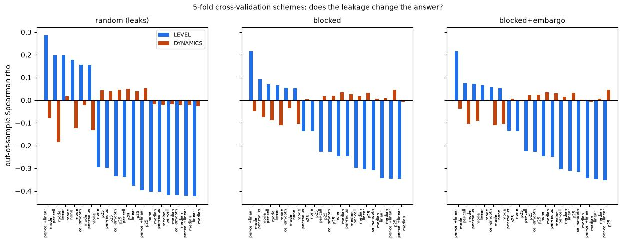
\includegraphics[width=\textwidth]{figures/w9_cv.pdf}
\caption{Out-of-sample level and dynamics correlations for every correction and estimator,
under all three cross-validation schemes. Blue is level, red is dynamics. The statistic is
height-ordered, so a positive bar is the correct sign.}
\label{fig:cv}
\end{figure}

\paragraph{Result.} Two findings.

\begin{enumerate}
\item \textbf{The sign depends on the estimator.} The \emph{mode} is correctly signed out of
sample ($+0.053$ uncorrected, $+0.217$ with the best correction). The \emph{median} is
\textbf{inverted}, at $-0.347$ to $-0.246$ across corrections. The project's ``inversion''
was measured on median-like statistics, and it is a property of \emph{those} statistics rather
than of the disparity field as a whole.
\item \textbf{No correction recovers the dynamics.} Across all eighteen combinations and all
three schemes the first-difference correlation stays within $\pm 0.11$ with no consistent
sign. The most expressive family tested --- a free offset per $20\times20$~px cell
\emph{plus} a plane, fitted on \SI{80}{\percent} of frames --- would recover a real signal
hiding under a fixed additive pattern. It does not.
\end{enumerate}

\noindent
\textbf{The static field is diagnosable and partly removable, and removing it does not recover
the dynamics.}

% =====================================================================================
\section{The shape mechanism}
\label{sec:shape}
% =====================================================================================

The estimator-dependence is not a defect of any statistic. It is a change in the disparity
distribution's \emph{shape}, and it is directly measurable.

\begin{table}[t]
\centering
\caption{The disparity distribution by regime. The dispersion is nearly unchanged while the
skewness collapses by \SI{84}{\percent}. The median and the mode respond to that change by
factors differing elevenfold in magnitude.}
\label{tab:shape}
\small
\begin{tabular}{@{}lS[table-format=2.3]S[table-format=2.3]S[table-format=+3.1]@{}}
\toprule
quantity & {low regime} & {high regime} & {change (\si{\percent})} \\
\midrule
median              & 12.340 & 14.500 & \textbf{+17.5} \\
mode                & 12.828 & 13.017 & +1.5 \\
\textbf{skewness}   & \textbf{2.583} & \textbf{0.421} & \textbf{-83.7} \\
kurtosis            & 45.887 & 30.095 & -34.4 \\
standard deviation  & 4.427 & 4.041 & -8.7 \\
\bottomrule
\end{tabular}
\end{table}

\begin{figure}[t]
\centering
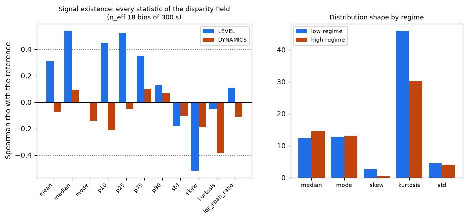
\includegraphics[width=\textwidth]{figures/w10_signal.pdf}
\caption{Left: every statistic of the disparity field against the reference, at \SI{300}{\second}
binning. No statistic survives correction. Right: the distribution's shape by regime.}
\label{fig:signal}
\end{figure}

Between regimes the \textbf{skewness collapses by \SI{84}{\percent}} while the dispersion is
nearly unchanged. A statistic that tracks the \emph{bulk} (the mode) and one that tracks
\emph{cumulative mass} (the median) must diverge when skewness changes: here the median moves
\SI{+17.5}{\percent} while the mode moves \SI{+1.5}{\percent}, an elevenfold difference in
response to the same physical change.

\paragraph{This unifies the synthetic and real results.} In the synthetic control the
disparity distribution has a \emph{fixed shape} across heights, so no statistic is biased by a
shape change and only the tail-sensitive rule fails --- which is exactly what was observed
(\texttt{lowest} errs by up to \SI{1471}{\metre} while \texttt{lowest\_mode} errs by at most
\SI{64}{\metre}). In the real atmosphere the shape \emph{does} change between regimes, so the
median and the mode diverge. One mechanism explains both, and the direction of the failure is
set by the sign of the skewness change.

% =====================================================================================
\section{The detection floor}
\label{sec:floor}
% =====================================================================================

We then asked whether \emph{any} statistic of the disparity field carries the reference's
temporal variation, once both series are resampled to a common independent grid. This is the
boundary question: if nothing does, no correction of the field can help.

\paragraph{Design.} Eleven statistics (mean, median, mode, $p_{10}$, $p_{25}$, $p_{75}$,
$p_{90}$, standard deviation, skewness, kurtosis and an IQR-to-span ratio) are computed over
\SI{300}{\second} bins --- the reference's own decorrelation time --- and each is correlated
with the \textbf{median of the reference over the same bin}. Eleven statistics against two
families of test is 22 comparisons, so a Bonferroni threshold is reported. The effective sample
size is computed from the lag-1 autocorrelation of the \emph{binned} series.

\paragraph{Result.} \textbf{No statistic reaches the corrected threshold.} The smallest
observed $p$ is $0.0063$ against a Bonferroni threshold of $0.00227$.

More importantly, the design itself is underpowered:

\begin{table}[t]
\centering
\caption{The detection floor. The observed correlations sit below what this session can
detect, so the experimental result is ``not detectable'', not ``absent''.}
\label{tab:floor}
\small
\begin{tabular}{@{}lr@{}}
\toprule
quantity & value \\
\midrule
binned series & 27 bins of \SI{300}{\second} $=$ \SI{2.25}{\hour} \\
effective sample size & $\neff = \mathbf{18.0}$ (one independent sample per \SI{449}{\second}) \\
\textbf{critical $|\rhoS|$ for significance} at $p = 0.05$ & \textbf{0.466} \\
$|\rhoS|$ detectable with \SI{80}{\percent} power at $\neff = 18.0$ & 0.731 \\
\textbf{$\neff$ needed for $\rhoS = 0.37$ at \SI{80}{\percent} power} & \textbf{60.3} \\
duration for a decisive session & $2.25~\text{h} \times (60.3/18.0) \approx \mathbf{7.5~\text{h}}$ \\
\bottomrule
\end{tabular}
\end{table}

The reference decorrelates over $\sim$\SI{267}{\second}, so 27 bins of \SI{300}{\second} hold
only \textbf{18 independent samples}, and the smallest detectable $|\rhoS|$ at $p=0.05$ is
\textbf{0.466}. \textbf{The dynamic signal, if it is present, lies at or below what this
session can detect} --- it is neither demonstrated nor excluded.


% =====================================================================================
\section{Supporting measurements}
\label{sec:supporting}
% =====================================================================================

Three further phases of work are recorded in the repository and support the results above.

\paragraph{Temporal alignment.} The image filenames are stamped in UTC and the ceilometer log
in Moscow time. An offset of exactly \SI{+3}{\hour} was established twice independently ---
once from the diurnal brightness envelope, and once by fitting the Sun's image azimuth with a
solar ephemeris, which matches to better than \ang{0.5} across \SI{14}{\hour}. Getting this
wrong by even one hour would have destroyed every correlation in
Section~\ref{sec:correction} silently, which is why it was confirmed by two methods rather
than one.

\paragraph{The static map.} The per-cell height field is largely a property of image position
rather than of time: the two halves of the session correlate at $r = 0.91$--$0.98$ while the
cloud moves. This is the observation that motivated Section~\ref{sec:static}.

\paragraph{Texture and sampling scale.} The median texture decorrelation length within the
crop is \SI{81.5}{px}, or \SI{229}{\metre} at \SI{2000}{\metre} --- that is, the cloud texture
is resolved by the imager with a comfortable margin, and the within-frame spread of the
disparity (\SI{2.13}{px} median) is not explained by an unresolved texture field. This rules
out a simple sampling-limit explanation for the dispersion.

\paragraph{The cloudless control.} The clear-sky day is used throughout as a discrimination
control rather than as ground truth: a method that returns a confident cloud signal under a
cloudless sky is inventing it. Two candidates were rejected for exactly this in
Section~\ref{sec:matcher}.

% =====================================================================================
\section{Methodological failures, and provenance assertions}
\label{sec:provenance}
% =====================================================================================

We report six defects found in our own harness as a first-class result, because they are the
most transferable finding in this work.

\begin{table}[t]
\centering
\caption{Six harness defects. None raised an exception. Two made the results look
\emph{more} significant than the truth, which is what allowed them to survive a review round.}
\label{tab:harness}
\scriptsize
\begin{tabular}{@{}p{0.03\textwidth}p{0.27\textwidth}p{0.60\textwidth}@{}}
\toprule
\# & defect & how it was caught, and what it cost \\
\midrule
1 & A validation metric scored below its own null & The metric maximised over a time shift and
  was compared against a null that did not; caught by computing the null the same way. \\
2 & Synthetic ground truth verified in the native frame while the consumer read the warped one
  & Caught by checking the frame the \emph{consumer} sees, not the one the producer wrote. \\
3 & Two call sites rendering ``the same'' cloud \ang{1.5} apart, because one passed a parameter
  and the other took a default & Cost \SI{551}{\metre} at \SI{2000}{\metre}; caught by
  reconciling two runs that should have agreed. \\
4 & A script asserting midway through three chained text replacements never reached its write,
  and exited \textbf{0} & The commit message described edits that were not in the file; caught
  by grepping the file afterwards rather than trusting the exit code. \\
5 & Random $k$-fold cross-validation on a series with lag-1 autocorrelation \SI{0.934}{} &
  Every held-out frame had near-duplicates in training; inflated the headline level result by
  $+0.070$. Caught by implementing blocked+embargo validation. \\
6 & A binned reference read from the sample nearest the bin's \emph{edge} rather than the median
  \emph{over} the bin & Manufactured a dynamic signal ($\rhoS=-0.37$, $p=0.038$) that vanished
  ($+0.095$, $p=0.667$) once corrected. Caught by asserting the reference's provenance. \\
\bottomrule
\end{tabular}
\end{table}

\paragraph{The meta-finding.} All six share a single mechanism:
\textbf{a quantity read from somewhere other than where it was claimed to come from.} They are
not arithmetic errors, and no unit test of a function's return value would have caught them,
because each individual value was correct; it was simply the \emph{wrong} value. Two of them
made the results look better, and defect~6 in particular produced a physically plausible,
correctly-signed signal that did not exist.

\paragraph{Provenance assertions.} We propose, implement and demonstrate a guardrail for this
class of defect: assertions that check \emph{where a value came from} rather than what it is
worth. Three are implemented in \texttt{src/clouds/validation/provenance.py}:

\begin{itemize}
\item \texttt{assert\_bin\_reference} --- a binned reference must equal the claimed aggregate
of the samples \emph{inside} the bin. Demonstrated to catch defect~6 on first execution.
\item \texttt{assert\_disjoint\_with\_embargo} --- no training frame may lie within the embargo
of \emph{any} held-out frame, resolved by binary search. Demonstrated to catch defect~5, and
it immediately caught a \emph{seventh} defect: our own embargo had been applied to the wrong
side of the split.
\item \texttt{autocorrelation\_report} --- lag-1 autocorrelation, decorrelation time and
$\neff$, so a cross-validation design can be checked against the series before it is trusted.
\end{itemize}

No guard can know whether a number is \emph{right}. Every one of these can know whether it came
from the right \emph{place}, and in this project that distinction was decisive.

% =====================================================================================
\section{Discussion}
\label{sec:discussion}
% =====================================================================================

\subsection{What is established}

\begin{enumerate}
\item The matcher, the fisheye geometry, the distortion model and the exact triangulation
recover a known height to \SI{0.072}{px} median error on a gated synthetic renderer.
\item The shipped \texttt{lowest} selection rule erred by \SIrange{325}{1471}{\metre} on
ground truth; \texttt{lowest\_mode} errs by at most \SI{64}{\metre} and is now the default.
\item The residual static field is dominated by a linear gradient in $u$ (\SI{66}{\percent})
rather than by a radial law (\SI{25}{\percent}), and largely cancels in height.
\item The estimator-dependence of the reported inversion is caused by a change in the
distribution's shape: skewness collapses by \SI{84}{\percent} while the dispersion is nearly
fixed.
\item No additive correction, over six families and three estimators, recovers the dynamics.
\item The instrument's dynamic capability is bounded by the detection floor: $\neff = 18$, a
critical $|\rhoS|$ of $0.466$, and \SI{7.5}{\hour} of data needed for a decisive test.
\end{enumerate}

\subsection{What is not established}

\begin{enumerate}
\item \textbf{The cause of the inversion is unattributed.} Twelve hypotheses were tested and
refuted; no mechanism we tested reproduces the specific signature (core $+1.5$~px, span
$\times2.2$, IQR $\times1.11$).
\item Whether the dynamic signal exists at all. It is below the detection floor of this
session; that is a statement about the experiment, not about the atmosphere.
\item Any statement about the \emph{level} of agreement beyond a single regime. There is a
level agreement in the low regime (\SI{2361}{\metre} against the ceilometer's
\SI{2250}{\metre}, $+111$~m), but the dynamics within that regime are wrong-signed.
\item Whether the anomaly is specific to this rig's disparity-starved geometry. Every
candidate is untested on a rig with a larger baseline.
\end{enumerate}

\subsection{Why this is a contribution}

A negative result is only useful if the instrument that produced it is known to be capable. We
supply the instrument's capability by construction, its limits by measurement, and its failure
by pre-registered refutation. The practical consequence is a clear map: the front end is sound,
the selection rule is fixed, the static field is characterised and partly removable, and the
remaining problem is either a physical effect not in our candidate set or a signal below the
detection floor.

\subsection{Threats to validity}

\paragraph{One session.} Every cross-validation fold is a time block within a single day, so
the folds are not independent in the way folds over independent days would be. This is the
single largest limitation, and it is the reason the detection floor is the binding constraint.

\paragraph{Footprint mismatch.} The camera footprint is \SI{1956}{\metre} at
\SI{1837}{\metre}; the ceilometer samples a column of order \SI{10}{\metre}. The ratio is
$\sim 200{:}1$. A level comparison between the two measures different things, and part of the
dispersion attributed to ``shape change'' may be genuine spatial variability within the camera
footprint.

\paragraph{Assumed baseline.} The \SI{45}{\metre} baseline is taken as given; no site
survey was available. An error in $B$ would scale all heights uniformly and would not produce
a sign inversion, but it would bias the level comparison.

\paragraph{Absence of meteorology.} No wind, temperature profile or site coordinates were
available, so no independent check on cloud motion or layer identity was possible.

% =====================================================================================
\section{Conclusion}
\label{sec:conclusion}
% =====================================================================================

We built a passive stereo cloud-base-height estimator, validated it by construction to
\SI{0.072}{px} median accuracy on known ground truth, found and fixed a selection-rule defect
costing up to \SI{1471}{\metre}, and then discovered that on real data the instrument does not
recover cloud base height.

We tested twelve explanations with pre-registered criteria and refuted all twelve. We
characterised the residual static field, showed that it is a $u$-gradient rather than a radial
law, and showed by cross-validated search that removing it does not recover the dynamics. We
identified the estimator-dependence of the reported inversion as a skewness-collapse effect
that unifies the synthetic and real results. And we established that the instrument's dynamic
capability is bounded by the detection floor of the experimental design --- not by an absence
of signal, but by an absence of \emph{samples}.

The cause of the inversion remains unattributed. The honest statement of the boundary is that
the dynamic signal, if present, is at or below what this session can detect.

\paragraph{What would settle it.} Three experiments, in increasing cost:

\begin{enumerate}
\item \textbf{A session long enough to detect $\rhoS = 0.37$.} The question is sample-limited:
$\neff = 18$ against a requirement of $60$, i.e. about \SI{7.5}{\hour} of binned data roughly
three times the present duration. This is the cheapest decisive experiment remaining, and it
converts ``below the detection floor'' into either a detection or a genuine absence.
\item \textbf{A footprint-matched reference.} A co-located radar or scanning lidar would remove
the $200{:}1$ sampling mismatch that makes a level comparison between a point column and a
\SI{2}{\km} area difficult to interpret at all.
\item \textbf{A rig with a larger baseline}, to test whether the anomaly is a property of a
disparity-starved geometry or of the method.
\end{enumerate}

\paragraph{A methodological recommendation.} The six harness defects reported here all shared
one mechanism, and none was detectable from a function's return value. We recommend
\emph{provenance assertions} --- checks that a value came from where it is claimed to have come
from --- as a standard guardrail in computational remote sensing, alongside the usual checks
on value, units and shape.

% =====================================================================================
\section*{Reproducibility}
\addcontentsline{toc}{section}{Reproducibility}
% =====================================================================================

Code, configuration and machine-readable results are in the repository at
\texttt{github.com/VanUST/clouds\_level\_research} (branch \texttt{dev}). The measurement data
are not redistributed. Every number in this paper is traceable to an artefact:

\begin{table}[h]
\centering
\small
\begin{tabular}{@{}ll@{}}
\toprule
result & artefact \\
\midrule
synthetic renderer and its gate & \texttt{experiments/w7/w7\_renderer.py}, \texttt{w7\_gate0.json} \\
matcher recovery on ground truth & \texttt{experiments/w7/w7\_control.json} \\
selection-rule defect & \texttt{experiments/w7/W7\_RESULT\_FINAL.md} \\
cross-validated correction search & \texttt{experiments/w9/w9\_cv.py}, \texttt{w9\_cv.json} \\
signal existence and shape mechanism & \texttt{experiments/w10/w10\_signal.py}, \texttt{w10\_signal.json} \\
provenance guards & \texttt{src/clouds/validation/provenance.py} \\
full record and all refutations & \texttt{docs/plan/research-workplan.md} \\
the twelve refutations in full & \texttt{docs/results/negative-results.md} \\
harness post-mortem & \texttt{experiments/w10/CODE\_REVIEW.md} \\
\bottomrule
\end{tabular}
\end{table}

\noindent
The synthetic controls, the pre-registered criteria and the negative results are retained in
the repository deliberately: they are the evidence that the null result is a measurement rather
than a failure.

\end{document}
